\subsection{Results}

Figures \ref{fig:dfsa}, \ref{fig:sfda} show the profiling results for the update rate of the Vanishing Point algorithm for different CPU-GPU allocations of the 3 tasks and different frequencies of the CPU and the GPU. Note, the CPU can be clocked upto 2.32 GHz (on all 4 cores), while the GPU can be clocked upto 0.852 GHz. We select 6 operating frequencies evenly spaced from the minimum and maximum Jetson CPU and GPU frequencies for both the CPU and the GPU. Also note that in these figures, Note, the 3 alphabet combinations imply the resource allocated to the Blur, Canny and Hough transform tasks respectively, e.g. C G C means that the Blur was on the CPU, Canny on the GPU and the Hough transform no the CPU and so on.


\begin{figure}[hbtp]
\centering
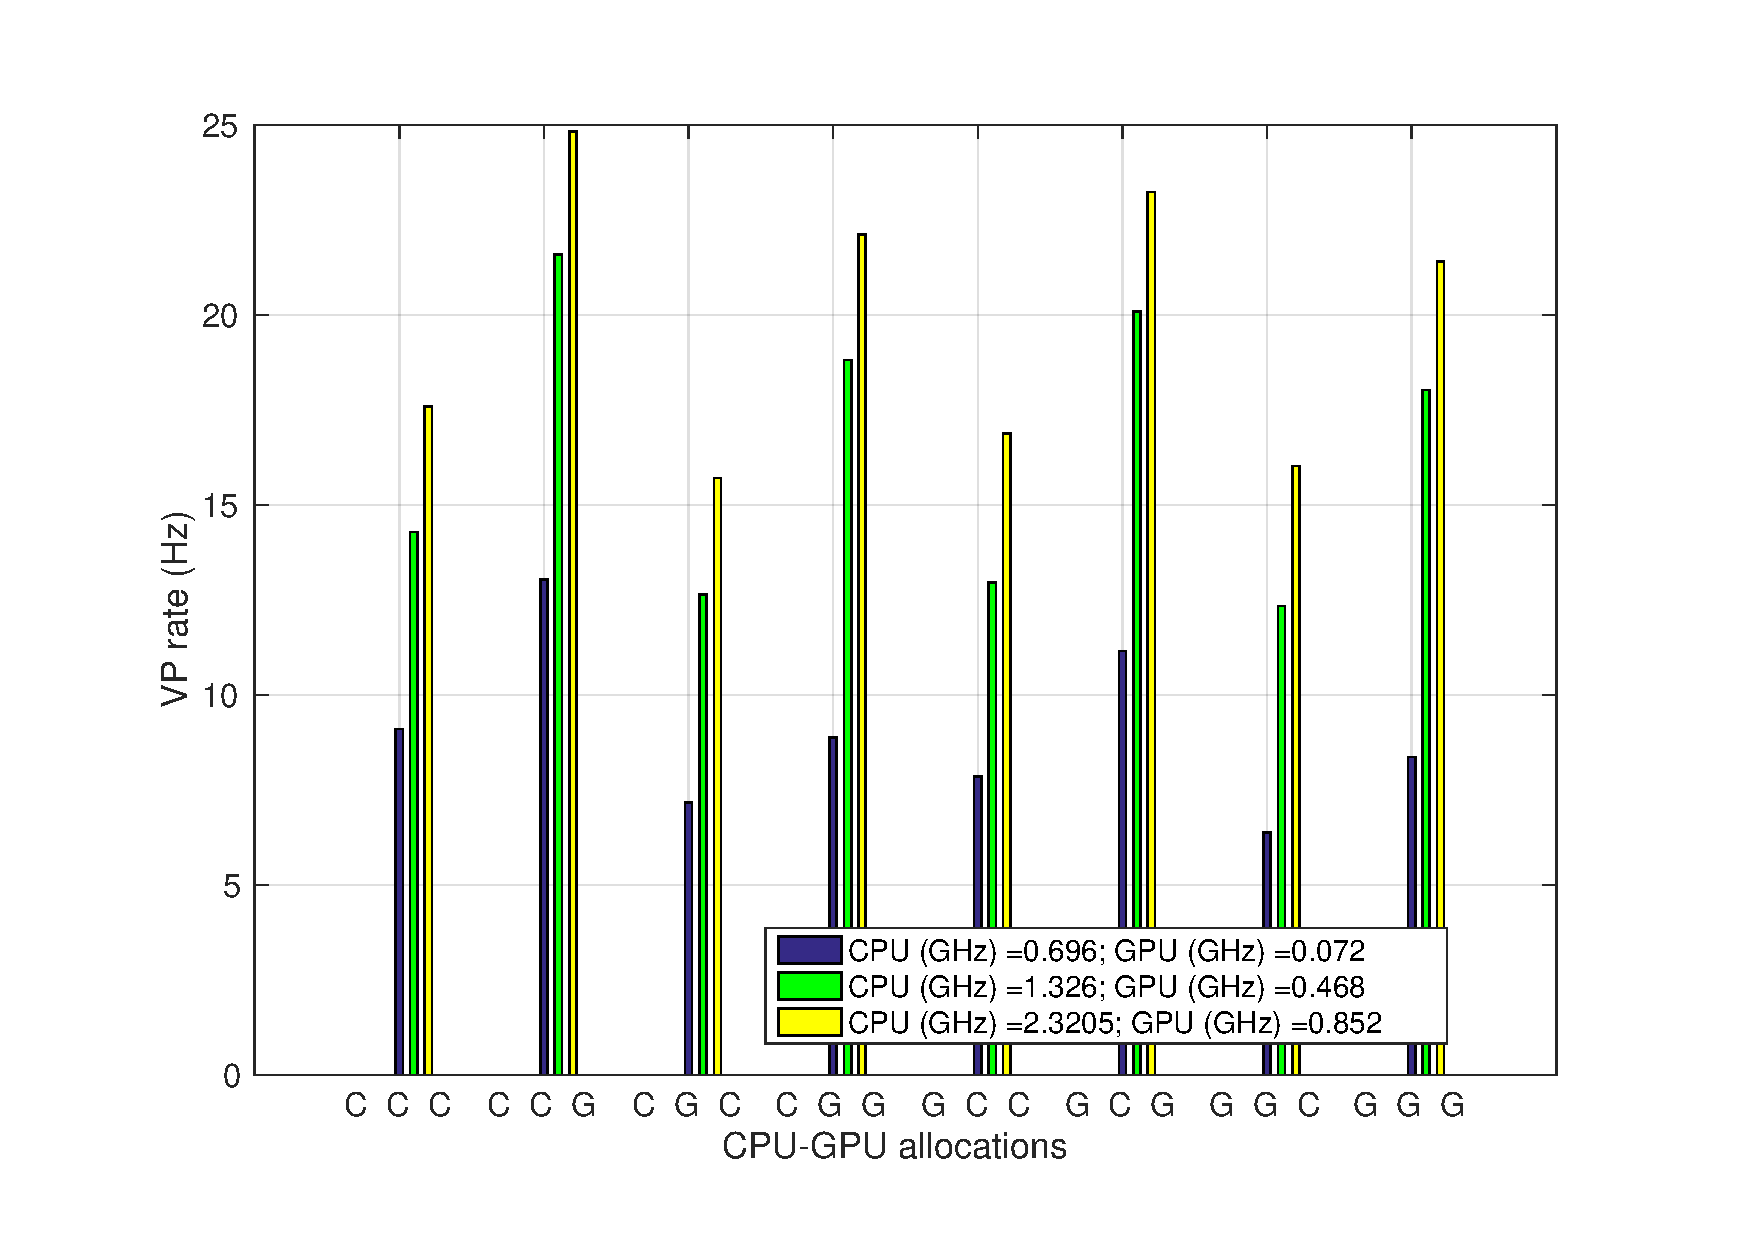
\includegraphics[width=0.46\textwidth]{Data/figs/RateHist.pdf}
\caption{Update rate for different frequencies and a given CPU-GPU assignment. For brevity we only consider 3 CPU and GPU frequencies for this figure, ranging from the minimum and maximum of both the CPU and the GPU. }
\label{fig:dfsa} %diff freq same assignment}
\end{figure}

\begin{figure}[htbp]
	\centering
	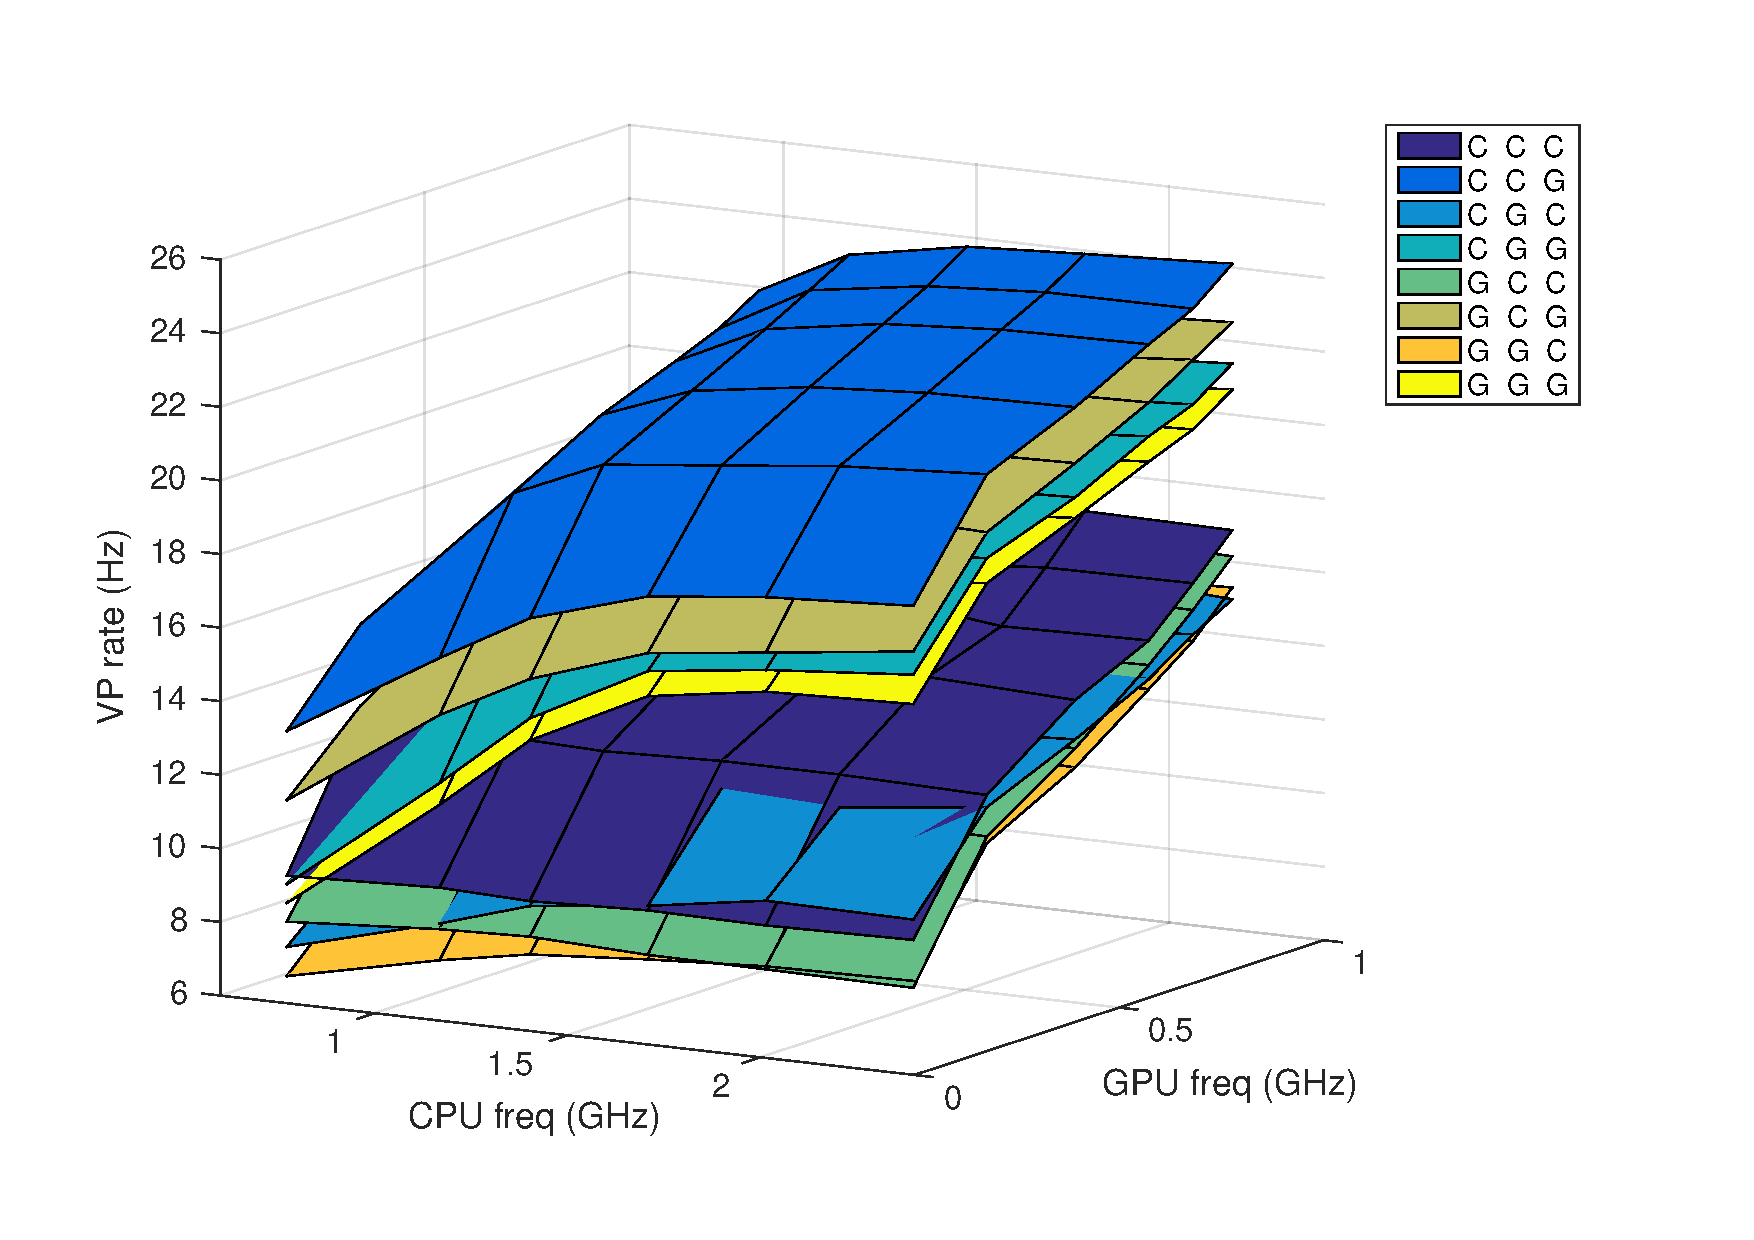
\includegraphics[width=0.46\textwidth]{Data/figs/surf_Rate.pdf}
	\caption{Update rate for different CPU-GPU assignments at fixed frequencies.}
	\label{fig:sfda}%same freq diff assignment}
\end{figure}

Figures \ref{fig:dfsa_pow}, \ref{fig:sfda_pow} show the profiling of average power consumed during the computations for the vanishing point over all frames in the video used for the profiling.


\begin{figure}[htbp]
\centering
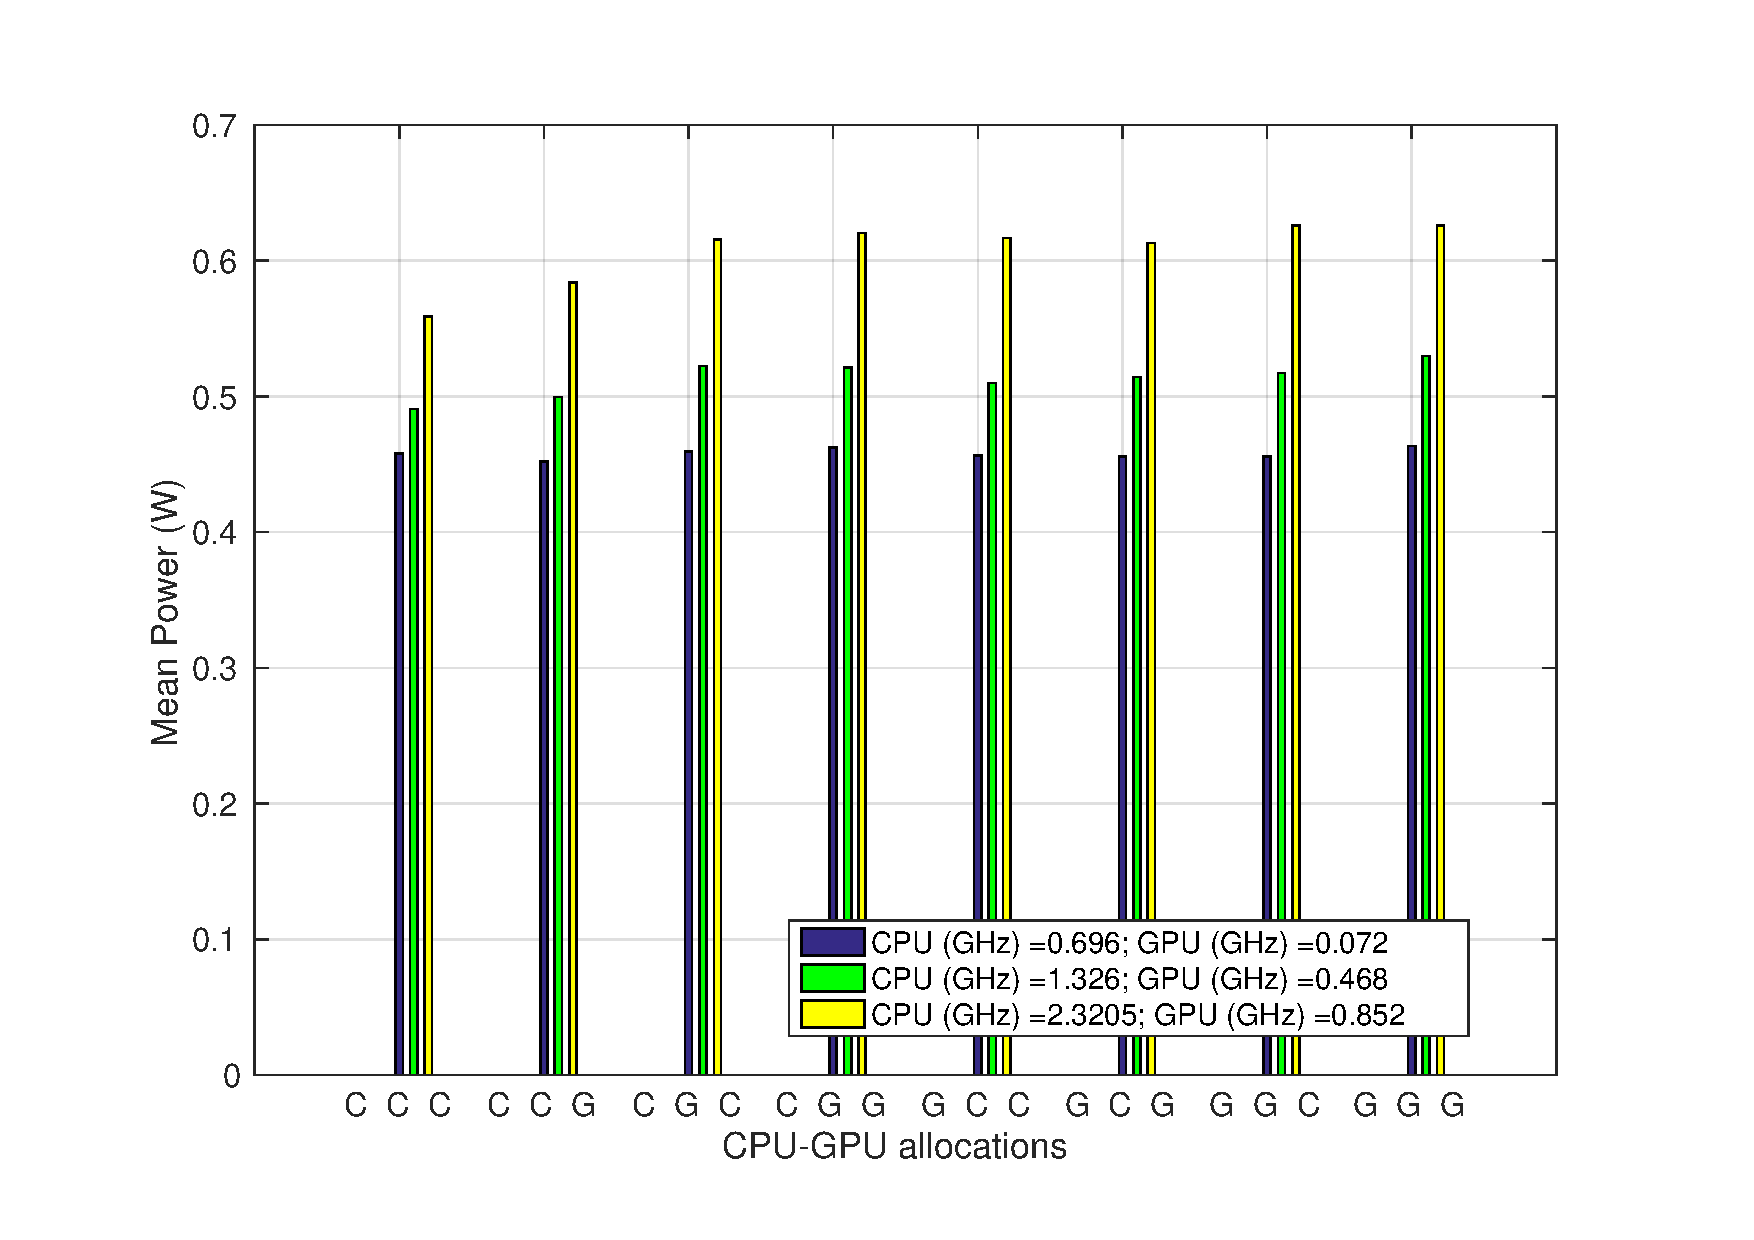
\includegraphics[width=0.46\textwidth]{Data/figs/PowerHist.pdf}
\caption{Mean Power consumed by the Jetson for different frequencies and a given CPU-GPU assignment.  For brevity we only consider 3 CPU and GPU frequencies for this figure, ranging from the minimum and maximum of both the CPU and the GPU.}
\label{fig:dfsa_pow} %diff freq same assignment}
\end{figure}

\begin{figure}[htbp]
	\centering
	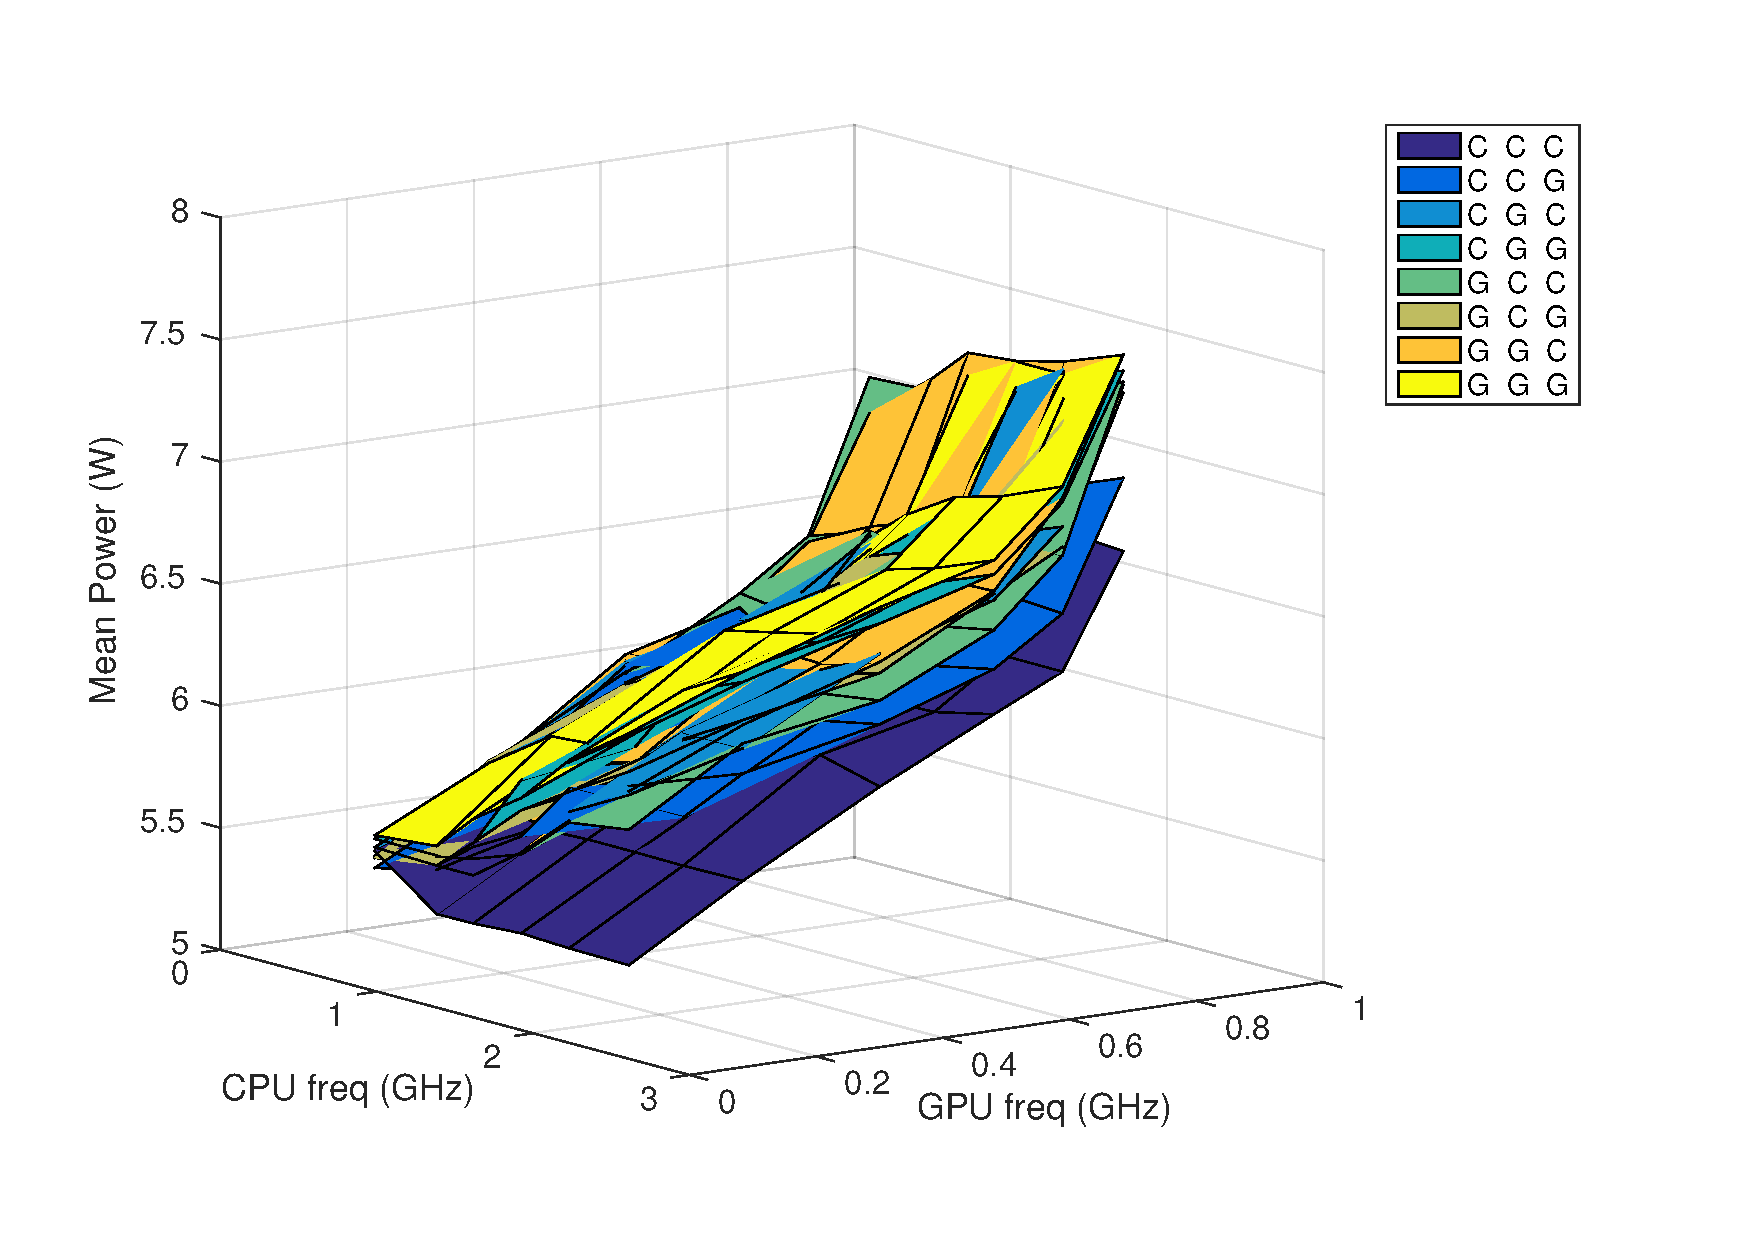
\includegraphics[width=0.46\textwidth]{Data/figs/surf_Power.pdf}
	\caption{Mean Power consumed by the Jetson for different CPU-GPU assignments at fixed frequencies.}
	\label{fig:sfda_pow}%same freq diff assignment}
\end{figure}


